\section{Introduction} \label{introduction}
%% General Introduction
In machine learning applications, a pipeline, a series of complex data processing steps, processes a labeled training dataset and produces a machine learning model.
The machine learning model is then used to make predictions on new unlabeled data.
The model then has to be deployed into an environment where it can answer prediction queries in real-time.

%% Intro to the problem of continuous improvement
After the model is deployed, new training data may become available.
Online learning methods are utilized to further train the deployed model.
In online learning, the model is updated based on the incoming data points.
Online learning can adapt the model to the new training data and provide an up-to-date model.
However, updating a model based on the individual data points may introduce instability.
Therefore, to guarantee the same level of quality as the offline batch training, online learning has to be highly tuned to the specific use case \cite{ma2009identifying, macmahan2013}.
One common method to alleviate the problem of low model quality is to perform periodical offline batch retraining over the existing and newly available data.
One of the challenges in many real-world use cases is the size of the training datasets.
Typically, training datasets are extremely large and require hours of data preprocessing and training to result in a new model.
Therefore, it is not feasible to train a new model frequently.
This results in a trade-off between the model training cost and the model quality.

Another challenge in the deployment of machine learning models is that incoming prediction queries and training data has to be first preprocessed by the same pipeline that is used to train the model.
Therefore, deploying models alone is not adequate and the entire pipeline has to be deployed as well.

%% Current Deployment Systems
\todo[inline]{Tilmann: What kind of platforms are the others then and why mention them at all? Behrouz: All of them are deployment platforms but only tensor flow allows pipelines to be deployed with the model as well. The rest only deploy the model.}
Several existing platforms such as Velox, Clipper, and TensorFlow Extended provide support for the deployment of models with TensorFlow Extended being the only one that supports the deployment of the entire machine learning pipeline \cite{crankshaw2014missing, crankshaw2016clipper, agarwal2014laser, baylor2017tfx}.
To maintain the quality of the model, existing systems support online learning, manual or automatic periodical retraining, or a combination of the two.
In many cases, the amount of training data is very large, thus training a new pipeline may take hours or even days \cite{baylor2017tfx}.

During the retraining, prediction queries are answered by the old model and new training data are accumulated.
For large datasets, by the time the retraining is finished, enough data is accumulated to prompt for a new periodical retraining.
As a result, in current deployment platforms, the deployed models are constantly stale.

\todo[inline]{I don't fully understand the figure. How is the retrained model deployed? with the preprocessing and batch training phase? Do the different types of arrows have specific meaning? If yes, what meaning do they have?}
%% Use case
\begin{figure}[h!]
\centering
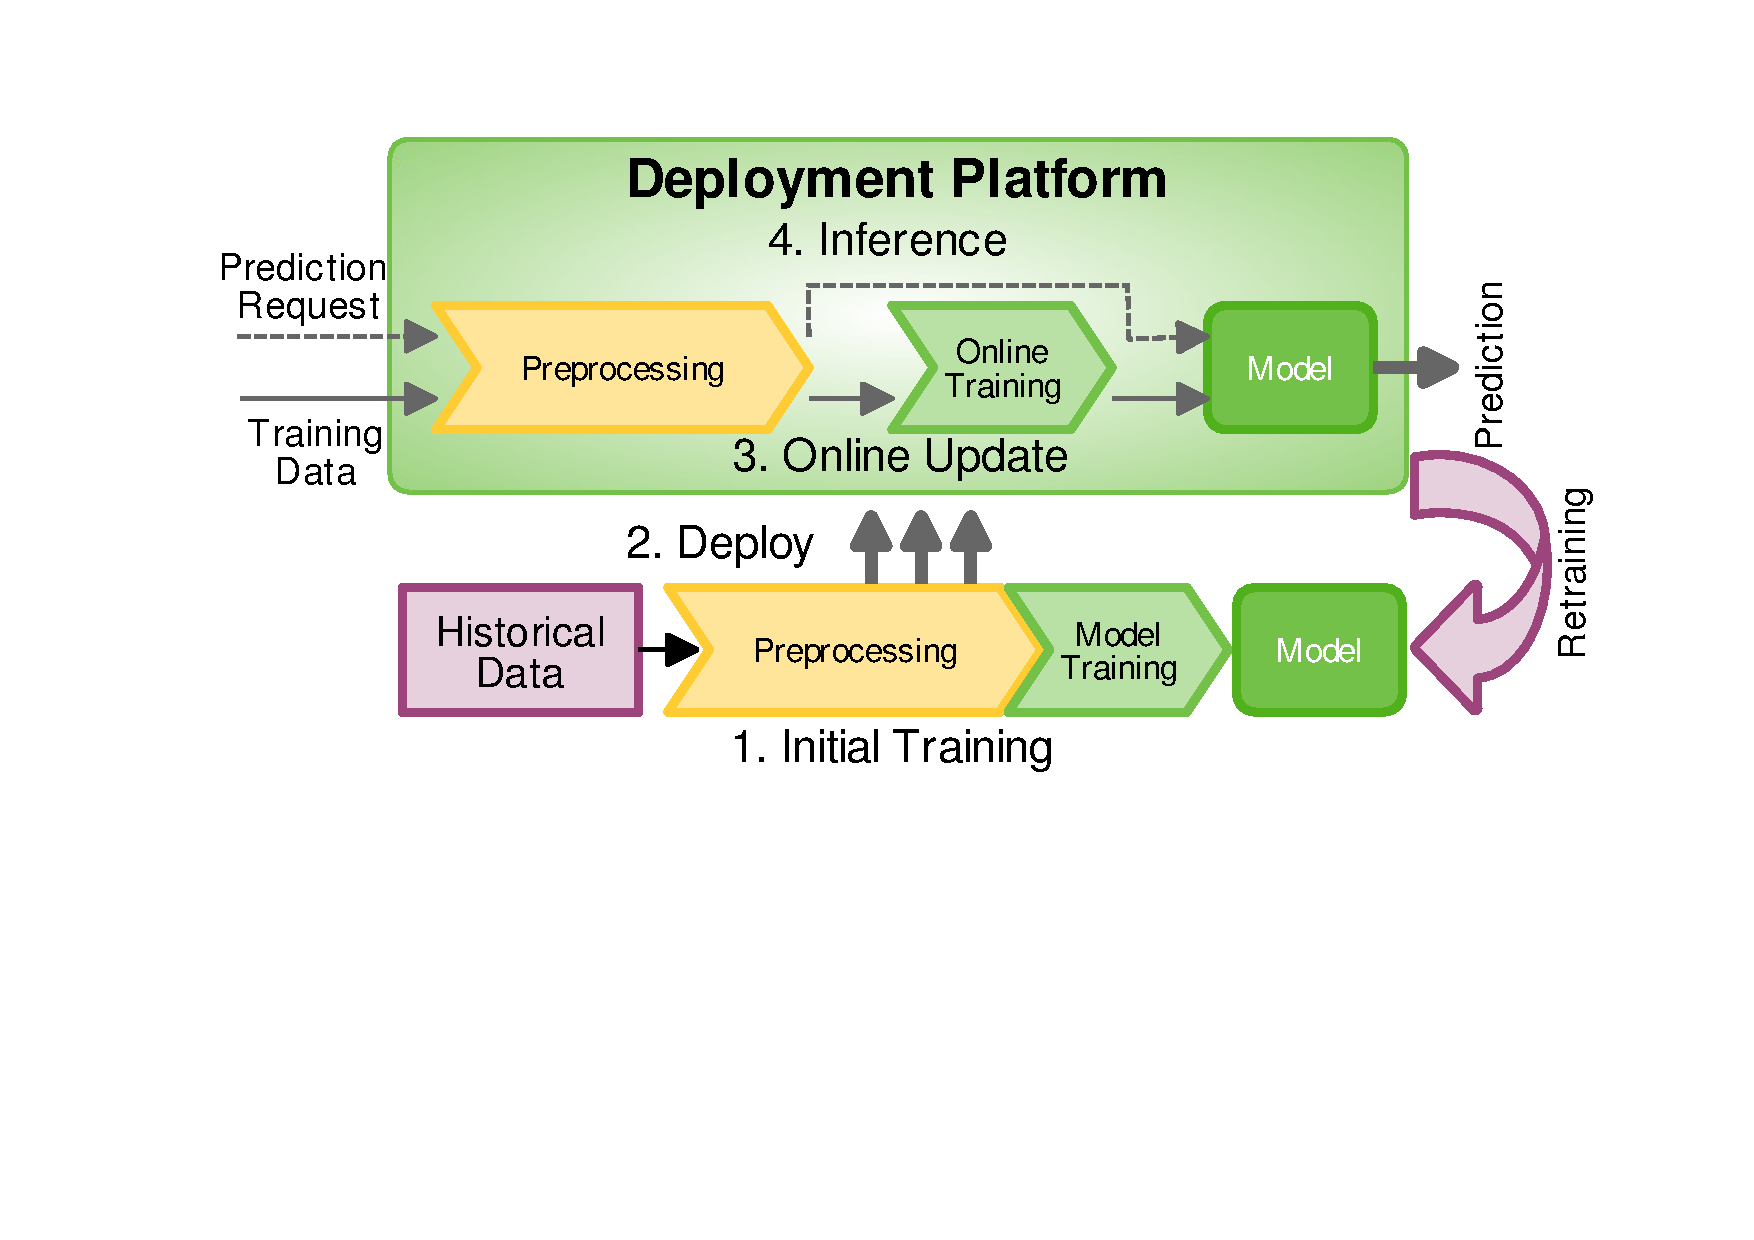
\includegraphics[width=\columnwidth]{../images/generic-motivational-example-v2.pdf}
\caption{Deployment process of machine learning pipelines}
\label{fig:motivational-example}
\end{figure}

Figure \ref{fig:motivational-example} shows the typical deployment process of existing systems.
During the initial training step, a user designs a machine learning pipeline that consists of several data and feature preprocessing steps and trains a machine learning model by utilizing a batch training algorithm.
Then in the deployment step, the model and the pipeline are deployed into the deployment platform.
To perform inference, the deployment platform directs the incoming prediction queries through the preprocessing steps.
Using the preprocessed features, the model makes a prediction.
During the online update phase, the deployment platform directs the data through the preprocessing steps of the pipeline and then, using an online training algorithm, the platform updates the model.
Finally, the deployment platform accommodates periodical retraining of the pipeline by either automatically initiating a batch training or prompting users to train and redeploy a new model to the deployment platform.
During the periodical retraining, the deployment platform disables the online updating of the model.

Several real-world use cases follow the workflow described in Figure \ref{fig:motivational-example}.
One example is the problem of Ad click prediction \cite{macmahan2013}.
In Ad click prediction, the machine learning pipeline consists of extracting features from the users and ads. 
Logistic regression models perform well in this setting \cite{macmahan2013}.
Prediction queries consist of the user's information and a pool of available ads for displaying to the user.
Once a prediction is made, a set of ads, with highest prediction scores, are displayed to the user.
Based on the action of the user (click or no click), new training data will be generated which is sent to the deployment platform for further training of the model.
Aside from the generated training data, new ads and new users are constantly becoming available.
As a result, new models have to be periodically trained and redeployed into the deployment platform.

The above example demonstrates the complexity and suboptimality of the deployment and maintenance of machine learning models and pipelines through periodical retraining.
Therefore, a flexible deployment platform should meet the model quality requirement without requiring the periodical retraining of the models and pipelines.

%% Our solution
We propose a deployment platform that continuously updates the model using a combination of the historical and incoming training data.
Similar to existing deployment platforms, our platform also utilizes online learning methods to update the model based on the incoming training data.
However, instead of periodical retraining, our deployment platform performs regular updates to the model based on samples of the historical data.
\todo[inline]{Alireza: Better to name them in this sentence. }
Our deployment platform offers two key optimizations, proactive training and online statistics computation and feature materialization. 

\textit{Proactive training.}
Proactive training is the process of utilizing samples of the historical data to update the deployed model.
First, the deployment platform processes a given sample using the pipeline, then it computes a partial gradient and updates the deployed model based on the partial gradient.
The updated model is immediately ready for answering prediction queries.
Unlike periodical retraining, each proactive training is very fast (similar to one iteration of offline training) and does not require the deployment platform to disable the online update.
Our experiments show that proactive training of the model achieves a lower error rate over time and requires fewer resources when compared to the periodical retraining.

\textit{Online Statistics Computation and Feature Materialization.}
Before updating the model using proactive training, the pipeline has to process the training data.
Every component of the pipeline needs to scan the data, updates the statistics (for example the mean and standard deviation of the standard scaler component), and finally transform the data.
Computing these statistics and transforming the data are time consuming processes.
Aside from the proactive training, our deployment platform also employs online learning methods to update the model in real-time.
During the online training, the deployment platform has to direct the data through the pipeline before updating the model.
During the online learning, we compute the required statistics and transform the data.
The deployment platform stores the updated statistics for every pipeline component and materializes the transformed features by storing them in memory or disk.
By reusing the computed statistics and the materialized features during the proactive training, we eliminate the data preprocessing steps of the pipeline and decrease the proactive training time.

% Our contributions
In summary, our contributions are:
\todo[inline]{Alireza: One could see this (the first contribution) as a higher level version of the second contribution. Is that the case ? Behrouz: True, but the first contribution is mostly about the platform itself that allows a pipeline to deployed, prediction queries to be send to the pipeline and model, and the model quality to be measured ... }
\begin{itemize}
\item A framework for continuously training deployed machine learning models and pipelines that adapts to the changes in the incoming data.
\item Proactive training of the deployed models and pipelines that frequently updates the model in-place using a combination of the historical and the incoming data which guarantees high-quality models.
\item Efficient pipeline processing and model training by online statistics computation and feature materialization, thus guaranteeing the availability of up-to-date models for answering prediction queries.
\end{itemize}

The rest of this paper is organized as follows:
Section \ref{continuous-training-serving} describes the details of our continuous training approach.
In Section \ref{sec:system-architecture}, we introduce the architecture of our deployment framework.
In Section \ref{evaluation}, we evaluate the performance of our continuous deployment approach.
Section \ref {related-work} discusses the related work.
Finally, Section \ref{conclusion} presents our conclusion and the future work.